\hypertarget{_result_scene_8cpp}{}\section{C\+:/\+H\+A\+L/\+P\+G関係/03\+\_\+作成プログラム/03\+\_\+\+H\+A\+L授業/就職作品/\+Project/source/02\+\_\+\+Scene/\+Scenes/\+Result\+Scene/\+Result\+Scene.cpp ファイル}
\label{_result_scene_8cpp}\index{C\+:/\+H\+A\+L/\+P\+G関係/03\+\_\+作成プログラム/03\+\_\+\+H\+A\+L授業/就職作品/\+Project/source/02\+\_\+\+Scene/\+Scenes/\+Result\+Scene/\+Result\+Scene.\+cpp@{C\+:/\+H\+A\+L/\+P\+G関係/03\+\_\+作成プログラム/03\+\_\+\+H\+A\+L授業/就職作品/\+Project/source/02\+\_\+\+Scene/\+Scenes/\+Result\+Scene/\+Result\+Scene.\+cpp}}


リザルトシーン\+Class  


{\ttfamily \#include \char`\"{}Result\+Scene.\+h\char`\"{}}\newline
Result\+Scene.\+cpp の依存先関係図\+:
\nopagebreak
\begin{figure}[H]
\begin{center}
\leavevmode
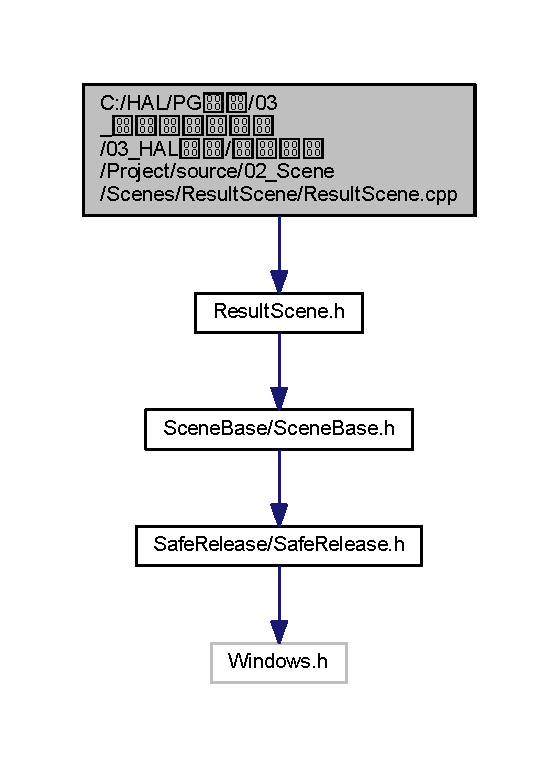
\includegraphics[width=268pt]{_result_scene_8cpp__incl}
\end{center}
\end{figure}


\subsection{詳解}
リザルトシーン\+Class 

\begin{DoxyAuthor}{著者}
Kai Araki 
\end{DoxyAuthor}
\begin{DoxyDate}{日付}
2018/07/24 
\end{DoxyDate}
